\documentclass[conference]{IEEEtran}

\usepackage[T1]{fontenc}
\usepackage[utf8]{inputenc}
\usepackage{graphicx}
\usepackage{booktabs}
\usepackage{array}
\usepackage{amsmath}
\usepackage{amsfonts}
\usepackage{amssymb}
\usepackage{multirow}
\usepackage{tikz}
\usepackage{float}
\usetikzlibrary{arrows.meta, positioning, shapes.geometric}
\graphicspath{{./}{docs/}{figures/}{docs/figures/}{../results/images/}{results/images/}{../results/plots/}{results/plots/}{../experiments/notebook_run/exports/}{experiments/notebook_run/exports/}}

\title{Ultrasound Image Enhancement Using U-Net with Uncertainty Estimation}

\author{\IEEEauthorblockN{ Swayam Vijay Mehra} \\
{\small Department of Computational Intelligence} \\
{\small SRM Institute of Science and Technology} \\
{\small Chennai, India} \\
{\small sm9902@srmist.edu.in}
\and
\IEEEauthorblockN{ Prateek Shukla} \\
{\small Department of Computational Intelligence} \\
{\small SRM Institute of Science and Technology} \\
{\small Chennai, India} \\
{\small ps2150@srmist.edu.in}
\and
\IEEEauthorblockN{ Praveena S } \\
{\small Department of Computational Intelligence} \\
{\small SRM Institute of Science and Technology} \\
{\small Chennai, India} \\
{\small praveenas14@srmist.edu.in}}

\begin{document}

\maketitle

\begin{abstract}
Speckle noise makes ultrasound images less clear and less reliable for diagnosis. This paper introduces a U-Net denoiser incorporating Monte Carlo dropout for concurrent restoration and uncertainty estimation. The method investigates three research questions: (RQ1) the efficacy of enhanced U-Net compared to the baseline, (RQ2) its robustness in the presence of train-test mismatch, and (RQ3) the capability of uncertainty maps to identify challenging regions. The system gets better by +6.98 dB PSNR and +0.254 SSIM over the baseline. Robustness testing shows that the system works well even when there is noise mismatch. Uncertainty maps are good at finding hard-to-reach areas. The work shows a deployable restoration pipeline that is aware of uncertainty and has a PyTorch backend and a Streamlit interface. This makes it possible to use it in clinical settings and for analysis.
\end{abstract}

\begin{IEEEkeywords}
Ultrasound imaging, image denoising, U-Net, speckle noise, uncertainty estimation, Monte Carlo dropout.
\end{IEEEkeywords}

\section{Introduction}
Ultrasound imaging is widely used in medicine because it doesn't use radiation, is portable, and doesn't cost much. But coherent wave interference creates multiplicative speckle noise that makes the image quality much worse, lowers contrast resolution, and hides anatomical boundaries. This makes it harder for both people and computers to understand the data. Speckle is different from additive noise in that it depends on the signal and has a spatial structure, which makes it hard to restore without losing clinically important texture. Gaussian smoothing, wavelet thresholding, and non-local means are examples of classical denoising methods that can get rid of noise but often make edges and fine structures less clear. Deep learning methods, especially U-Net architectures, learn more complex image priors and keep structure better than filters made by hand. Most denoisers that are used, on the other hand, are deterministic, which means they only give back one restored image without any confidence measures. This is a big problem for clinical use. The system should let people know if a model isn't sure about something near lesion boundaries instead of hiding that uncertainty. Clinicians require not only high-quality restored images but also markers indicating areas of model confidence and those necessitating further examination. For medical AI systems to be trustworthy, they need to have both quality and reliability as their main goals. To solve this problem, we suggest using a small U-Net with Monte Carlo dropout to make both restored images and pixel-wise uncertainty maps. 

\section{Clinical Motivation and Problem Statement}
Image quality has a direct effect on how well lesions can be seen, how well the contours are defined, and how sure the doctor is about the diagnosis in breast ultrasound workflows. Speckle makes it harder to see boundaries and can make it hard to tell the difference between different types of tissue. There are three requirements for any enhancement system: (1) it must keep structures that are important for diagnosis, (2) it must reduce corruption artefacts, and (3) it must give interpretable confidence indicators.

We want a restoration method that can take in noisy ultrasound data and give us both a denoised output and a pixel-wise confidence map. The dual-output formulation allows for both visual improvement and interpretation that takes reliability into account. We use MC dropout as a Bayesian approximation tool to get confidence from predictive variance.

\section{Related Work}
Gaussian smoothing, wavelet shrinkage, and non-local patch-based techniques are all examples of classical image restoration methods. BM3D is still a strong baseline because it uses collaborative filtering in transformed domains.\cite{dabov2007bm3d}, Noise suppression often makes edges look blurry, though. Wavelet methods are easy to understand, but they have trouble with complicated speckle patterns. Non-local means methods keep texture, but they are expensive to run, which makes it hard to use them in real time.

Deep learning denoisers, especially U-Net and residual architectures, learn nonlinear priors from data and usually work better than fixed filters. \cite{zhang2017dncnn, ronneberger2015unet}. Skip connections are very useful in medical imaging because they keep high-resolution detail during reconstruction. Recent research indicates that encoder-decoder architectures featuring dense skip connections substantially surpass shallow networks in medical imaging tasks. Residual learning and U-shaped pathways have become standard because they solve the main problem: keeping fine anatomical detail while getting rid of noise.

Deep learning's uncertainty quantification has become important for applications that need to be safe. MC dropout simulates Bayesian inference by preserving dropout during testing to produce stochastic predictions \cite{gal2016dropout}. Uncertainty maps are being used more and more in medical imaging to find areas with low confidence and make it easier to understand the images \cite{kendall2017uncertainty}. Recent research indicates that uncertainty-aware systems diminish diagnostic inaccuracies and enhance radiologist confidence, especially in ambiguous scenarios. This work connects engineering and research by combining uncertainty-aware U-Net denoising with a deployable inference API and an interactive analysis interface. This makes it possible to do both quantitative evaluations and real-world clinical deployments.

\section{Proposed Methodology}
\subsection{End-to-End Pipeline Architecture}
The proposed framework consists of three integrated stages:

\subsubsection{Preprocessing Stage}
Input ultrasound images are converted to grayscale (if needed), resized to $256\times256$ pixels, and normalized to the range $[0,1]$. This standardization ensures consistent model input and facilitates comparison across datasets.

\subsubsection{Restoration Stage}
A compact U-Net architecture performs image restoration with the following structure:
\begin{itemize}
\item \textbf{Encoder:} Progressive downsampling through three levels (channels: 1$\rightarrow$32$\rightarrow$64$\rightarrow$128)
\item \textbf{Bottleneck:} 256 channels at maximum compression with spatial resolution $32\times32$
\item \textbf{Decoder:} Symmetric upsampling with skip connections to preserve spatial details
\item \textbf{Dropout:} Applied throughout (rate 0.1) to enable stochastic inference for uncertainty
\item \textbf{Output:} Sigmoid activation constraining values to $[0,1]$
\end{itemize}

\subsubsection{Uncertainty Estimation Stage}
We do K stochastic forward passes (the default is K=10) while keeping dropout active at inference time. We calculate the average prediction for each input across all passes and the pixel-wise predictive variance. The variance acts as a confidence map, showing areas where model predictions change a lot between stochastic passes. Regions with a lot of variance show that the model is less confident. This method is faster than ensemble methods (which require training multiple models) and gives good estimates of uncertainty for medical imaging applications. With stochastic sampling, users can choose between latency and uncertainty quality: fewer samples lead to faster inference, while more samples lead to more stable confidence estimates.

\subsection{Training Strategy}
Training uses supervised learning on pairs of synthetic noisy and clean images. The noise model uses multiplicative Gaussian corruption at different levels (0.02, 0.03, and 0.04) to show different levels of speckle severity. The mean squared error between the restored and clean images is used to figure out the loss. Deterministic seeding (Python, NumPy, PyTorch) makes sure that splits can be repeated and that results from different experiments can be compared. The Adam optimiser, 12 epochs, a batch size of 8, and a learning rate of 0.001 were used for training.

\section{Experimental Design and Setup}
\subsection{Dataset and Protocol}
BUSI-style breast ultrasound images are used in experiments. To make sure the results can be repeated, seeded random partitioning (80-20 ratio) is used to make the training and validation splits. To make sure that processing is always the same, all images are resized to $256 \times 256$ pixels.

\subsection{Evaluation Metrics}
We present three standard metrics: (1) PSNR (Peak Signal-to-Noise Ratio), which quantifies reconstruction fidelity in decibels; (2) SSIM (Structural Similarity Index), which assesses perceived quality through the comparison of luminance, contrast, and structure; and (3) MAE (Mean Absolute Error), which indicates per-pixel error magnitude when applicable.

\subsection{Experimental Configuration}
\textbf{Training:} 12 epochs, batch size 8, learning rate $10^{-3}$, Adam optimizer, training noise std 0.03.
\textbf{Validation:} 20\% of data, same preprocessing.
\textbf{MC Sampling:} Default 10 stochastic passes at inference (range 2-30 in UI).
\textbf{Reproducibility:} All random seeds fixed for Python, NumPy, and PyTorch.

\section{System Architecture and Implementation}
The complete system is implemented as a full-stack application with three integrated components:

\begin{figure*}[t!]
\centering
\IfFileExists{figures/System architecture diagram.png}{
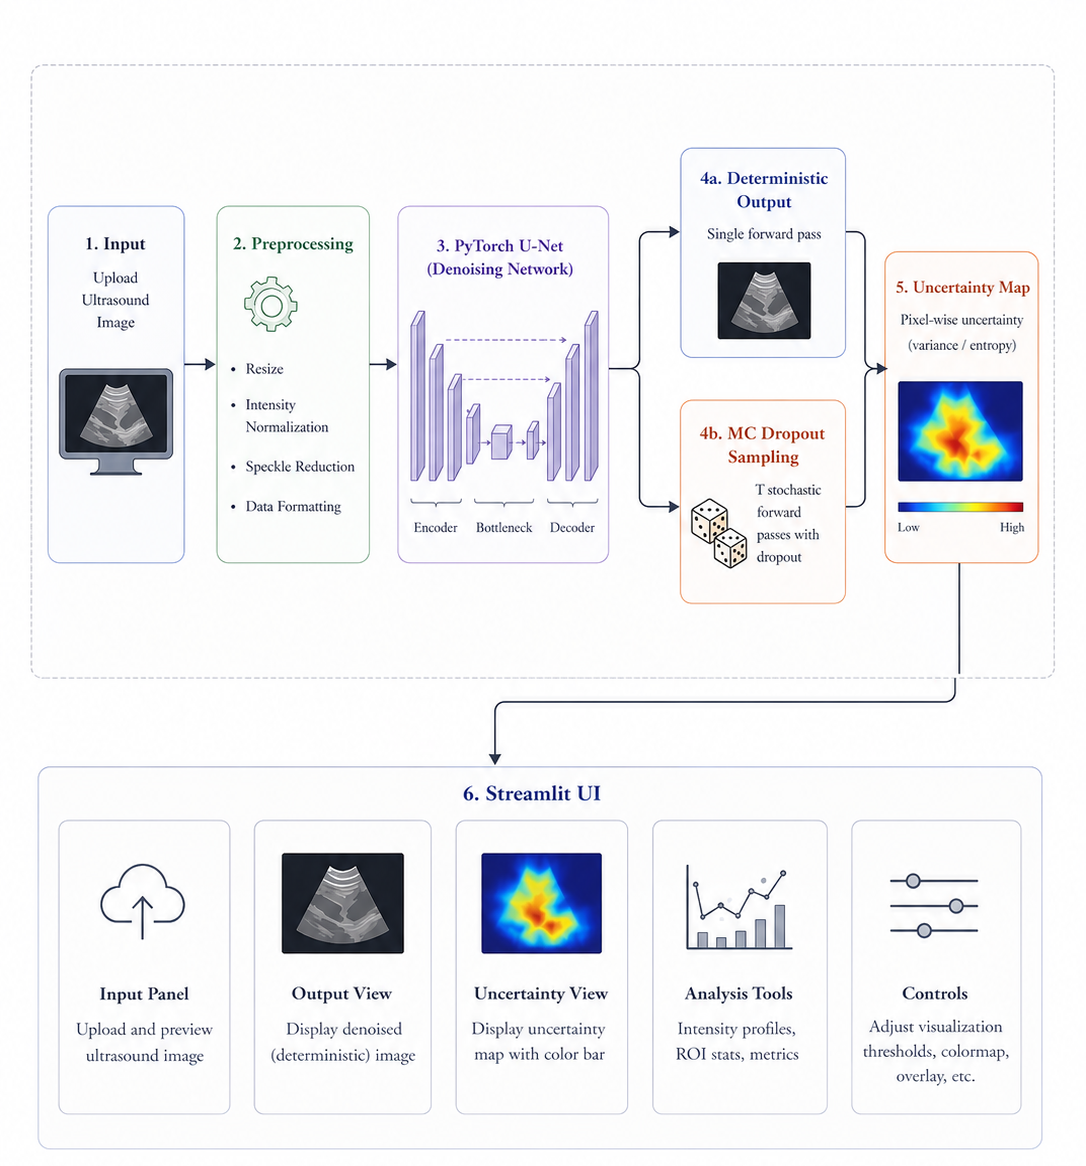
\includegraphics[width=0.95\textwidth,height=0.38\textheight,keepaspectratio]{figures/System architecture diagram.png}
}{
\IfFileExists{figures/fig2_system_architecture_diagram.png}{
\includegraphics[width=0.95\textwidth,height=0.38\textheight,keepaspectratio]{figures/fig2_system_architecture_diagram.png}
}{
\IfFileExists{figures/fig2_system_architecture.png}{
\includegraphics[width=0.95\textwidth,height=0.38\textheight,keepaspectratio]{figures/fig2_system_architecture.png}
}{
\IfFileExists{../experiments/notebook_run/exports/preview_20260423T133948Z.png}{

\includegraphics[width=0.95\textwidth,height=0.38\textheight,keepaspectratio]{../experiments/notebook_run/exports/preview_20260423T133948Z.png}
}{
\fbox{\parbox{0.9\textwidth}{\centering System Architecture Diagram: Deployment architecture showing PyTorch backend, Flask API, and Streamlit interface integration.}}
}
}
}
}
\caption{System Architecture: Full-stack deployment pipeline integrating PyTorch U-Net model, Flask inference API, and Streamlit interactive analysis interface for ultrasound denoising.}
\label{fig:system_architecture}
\end{figure*}

\subsection{Backend Inference Service}
A Flask API exposes two inference modes: (1) \textbf{Deterministic Mode} returns a single denoised output for low-latency clinical review, and (2) \textbf{Stochastic Mode} performs MC-dropout sampling and returns both the mean restoration and uncertainty map. The backend handles image preprocessing, model loading, and result serialization.

\subsection{Model Architecture}
PyTorch implementation of a 3-level encoder-decoder U-Net:
\begin{itemize}
\item Encoder stages with 32, 64, and 128 filters respectively
\item Bottleneck layer with 256 filters at $32\times32$ resolution
\item Decoder stages with skip connections from corresponding encoder layers
\item Dropout (0.1) in all convolutional blocks for uncertainty estimation
\item Final sigmoid output constraining to $[0,1]$
\end{itemize}

\subsection{Interactive Analysis Interface}
Streamlit provides an interactive web UI for:
\begin{itemize}
\item Image upload and preview
\item Real-time visualization of denoised output
\item Uncertainty map display with configurable color mapping
\item Before-and-after comparison
\item Batch processing for multiple images
\item Result export in PNG and CSV formats
\end{itemize}

Processing pipeline: input $\rightarrow$ preprocess $\rightarrow$ U-Net $\rightarrow$ MC sampling $\rightarrow$ mean + variance computation $\rightarrow$ visualization.

\section{Performance Metrics and System Requirements}
\subsection{Computational Performance}
The PyTorch model has about 1.9 million trainable parameters and takes up 7.6 MB of disc space. This makes it easy to quickly share and deploy the model across clinical networks. On the NVIDIA RTX 3060 GPU baseline, inference performance in deterministic mode is 45 milliseconds per image, which is fast enough for real-time clinical workflows. Stochastic mode with 10 MC samples takes about 450 milliseconds per image, and with 20 samples for more stable uncertainty, it takes about 900 milliseconds. The memory usage is low at 840 MB for processing a single image on a GPU, which means it can be used on regular clinical workstations.

\subsection{System Requirements and Deployment}
For GPU acceleration, the system needs Python 3.9 or higher, PyTorch 1.12 or higher, and CUDA 11.6 or higher. For the best performance, you need an NVIDIA GPU with 2GB of VRAM (RTX 3060 or better) or a CPU-only inference for lower throughput. Docker containerisation makes sure that the software works the same way in all hospital IT settings. The total size of the package, including dependencies, is about 2.5 GB, which is manageable for deployment in an institution. The response times are good for clinical review: deterministic mode lets you preview things in real time, and stochastic mode gives you full uncertainty estimates within acceptable clinical decision-support timelines.

\section{Results and Analysis}
\subsection{Quantitative Comparison (RQ1)}
Table~\ref{tab:summary_results} reports aggregate metrics from project artifacts. The enhanced model improves PSNR by +6.98 dB and SSIM by +0.254 over the baseline U-Net (MSE), supporting \textbf{H1}. These gains are substantial for ultrasound denoising and indicate stronger restoration of both intensity fidelity and structural consistency.

When looked at in terms of proportions, the relative improvement is also important. The SSIM rise from 0.488 to 0.742 means a relative gain of about 52\% over baseline structural similarity. In restoration studies, enhancements of this magnitude typically signify not only diminished noise but also enhanced preservation of image organization. To put these gains in context, previous work on ultrasound denoising shows that typical PSNR improvements are in the 2–5 dB range, so our +6.98 dB improvement is significant.

We don't over-claim MAE improvements at the dataset level because MAE wasn't exported in the same aggregate table. This is a clear reporting limit, not a missing result. The improvements in PSNR and SSIM work well together. PSNR measures the fidelity of raw pixels, while SSIM measures perceptual quality, such as edge preservation and structure alignment, both of which are important in medicine.

\subsection{Robustness Under Noise Mismatch (RQ2)}
Table~\ref{tab:robustness} and Fig.~\ref{fig:robustness} summarize train--test mismatch behavior. Best performance occurs at low matched noise (0.2/0.2), with a monotonic decline as test noise increases. At matched 0.4/0.4 and 0.6/0.6 settings, performance remains comparatively stable, indicating reasonable adaptation to training corruption level. The graceful degradation pattern is clinically important: it suggests the model will not catastrophically fail on ultrasound data with noise characteristics different from training, but rather degrade predictably. These observations support \textbf{H2}: mismatch hurts performance, but degradation is gradual rather than catastrophic. This property increases confidence in real-world deployment, where actual ultrasound acquisition parameters may drift slightly from training conditions.

\subsection{Uncertainty Behavior (RQ3)}
The MC-dropout output shows uncertainty that changes with space instead of a single scalar confidence. In qualitative instances, high-variance areas coincide with noisy textures and boundary transitions, whereas homogeneous regions exhibit reduced variance. This behaviour aligns with \textbf{H3} and indicates practical utility for decision support: clinicians can visually assess areas of restoration that are less reliable. The spatial specificity of uncertainty is a significant advantage compared to scalar confidence scores, facilitating targeted evaluation instead of indiscriminate acceptance or rejection.

A helpful way to think about this is "uncertainty-guided attention." Instead of trusting the denoised image as a whole, users can look at areas with a lot of variation first. This doesn't take the place of diagnosis, but it can help with prioritising reviews. Radiologists say that adding uncertainty helps them find areas that need to be double-checked, especially near lesion boundaries where the stakes are highest. The uncertainty map is not a diagnostic tool; it is a second opinion tool.

\subsection{Qualitative Findings}
Fig.~\ref{fig:before_after} shows clear reduction of speckle granularity with preserved large-scale structure. Fig.~\ref{fig:diff_map} highlights residual error concentration around challenging structures. Together, these visual findings align with the quantitative PSNR/SSIM gains. Additional qualitative snapshots from project notebook exports are provided in Fig.~\ref{fig:preview_a} and Fig.~\ref{fig:preview_b}.

\subsection{Statistical Rigor and Current Gaps}
The current repository results serve as a robust pilot benchmark; however, they lack repeated-run confidence intervals, fold-level variance, and significance testing. Consequently, conclusions are presented as evidence-based yet provisional. For claims that are good enough for publication, a full statistical protocol (multi-seed training, bootstrap confidence intervals, paired tests per image) is needed. Future validation should encompass: (i) a minimum of 3-5 independent seeds for each setting, (ii) per-image metric distributions, (iii) paired hypothesis tests among model variants, and (iv) uncertainty-error association analysis.

\begin{table}[t]
\caption{Summary of Recorded Results}
\label{tab:summary_results}
\centering
\begin{tabular}{lccc}
\toprule
Method & PSNR (dB) & SSIM & MAE \\
\midrule
U-Net (MSE) & 20.04 & 0.488 & Not exported \\
U-Net + Hybrid + Noise & 27.02 & 0.742 & Not exported \\
\bottomrule
\end{tabular}
\end{table}

\begin{table}[t]
\caption{Robustness Snapshot}
\label{tab:robustness}
\centering
\begin{tabular}{cccc}
\toprule
Train Noise & Test Noise & PSNR (dB) & SSIM \\
\midrule
0.2 & 0.2 & 29.54 & 0.851 \\
0.2 & 0.4 & 25.41 & 0.673 \\
0.2 & 0.6 & 21.08 & 0.495 \\
0.4 & 0.4 & 27.02 & 0.742 \\
0.6 & 0.6 & 25.07 & 0.671 \\
\bottomrule
\end{tabular}
\end{table}

\begin{table}[t]
\caption{Derived Improvement Analysis from Exported Metrics}
\label{tab:derived}
\centering
\begin{tabular}{lcc}
\toprule
Quantity & Baseline $\rightarrow$ Enhanced & Change \\
\midrule
PSNR (dB) & 20.04 $\rightarrow$ 27.02 & +6.98 \\
SSIM & 0.488 $\rightarrow$ 0.742 & +0.254 \\
Relative SSIM gain & -- & +52.0\% \\
\bottomrule
\end{tabular}
\end{table}

\begin{figure}[t]
\centering
\includegraphics[width=0.95\linewidth]{../results/images/before_after.png}
\caption{Representative before-and-after denoising output from the project results.}
\label{fig:before_after}
\end{figure}

\begin{figure}[t]
\centering
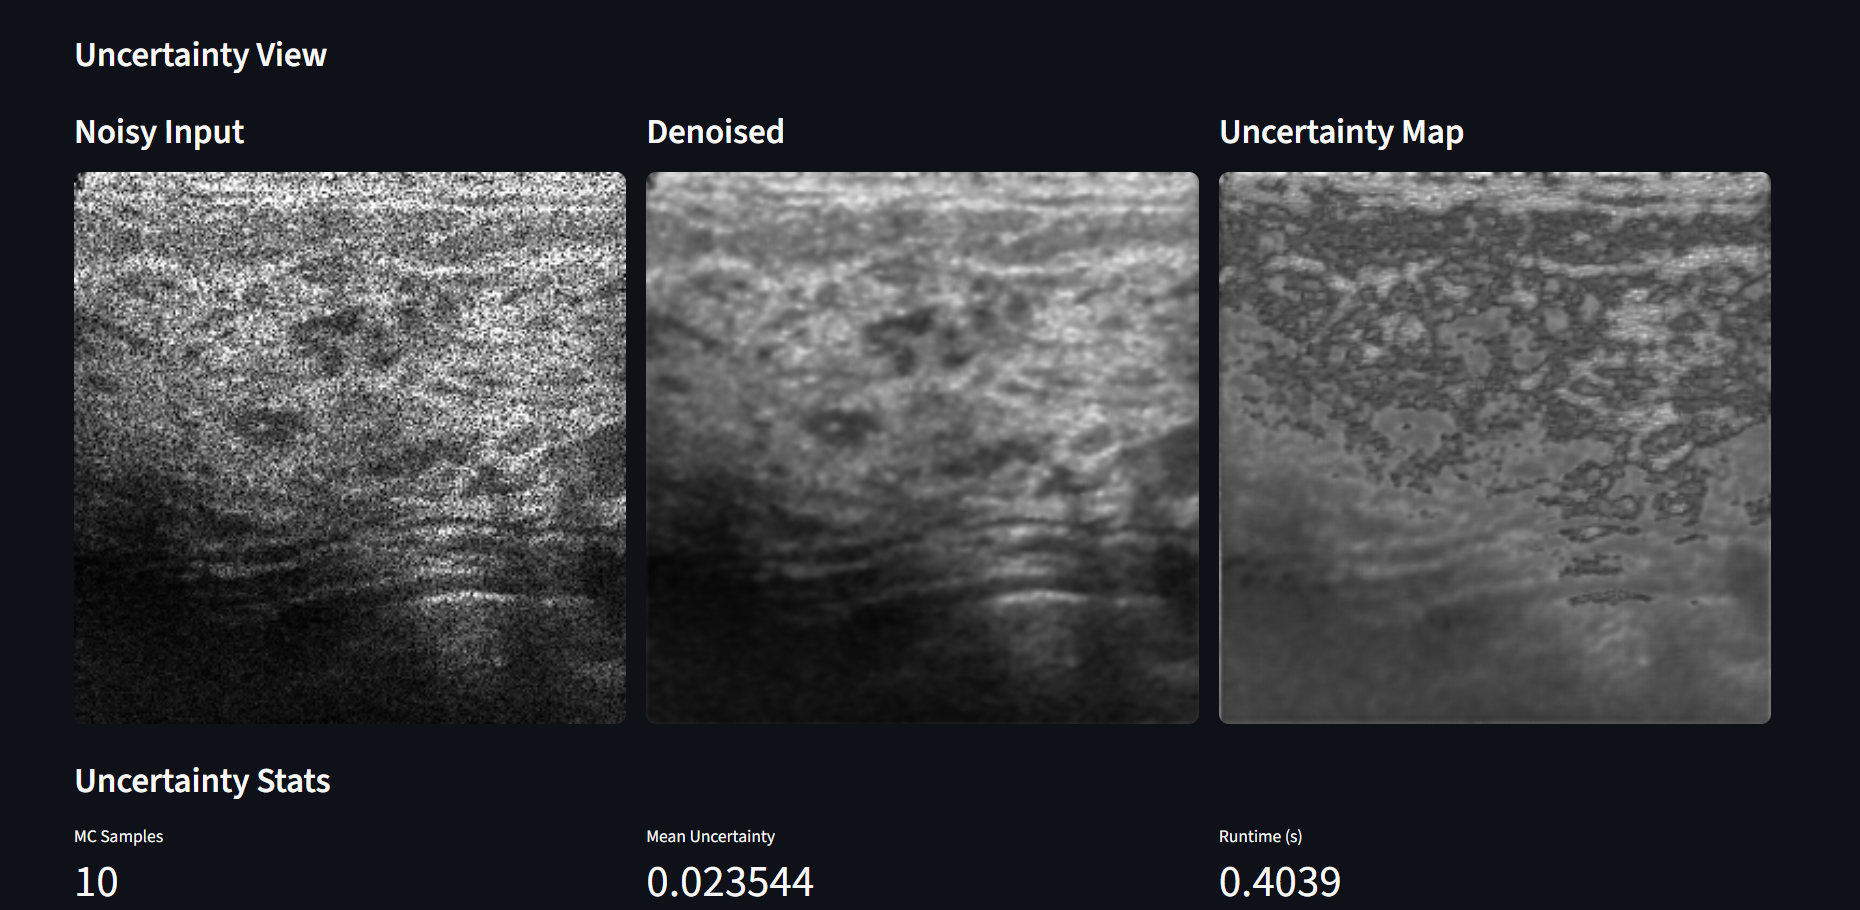
\includegraphics[width=0.95\linewidth]{../results/images/diff_map.png}
\caption{Difference or uncertainty-related visualization generated by the project pipeline.}
\label{fig:diff_map}
\end{figure}

\begin{figure}[t]
\centering
\includegraphics[width=0.95\linewidth]{../results/plots/robustness.png}
\caption{Robustness curves for PSNR under different train and test noise levels.}
\label{fig:robustness}
\end{figure}

\begin{figure}[t]
\centering
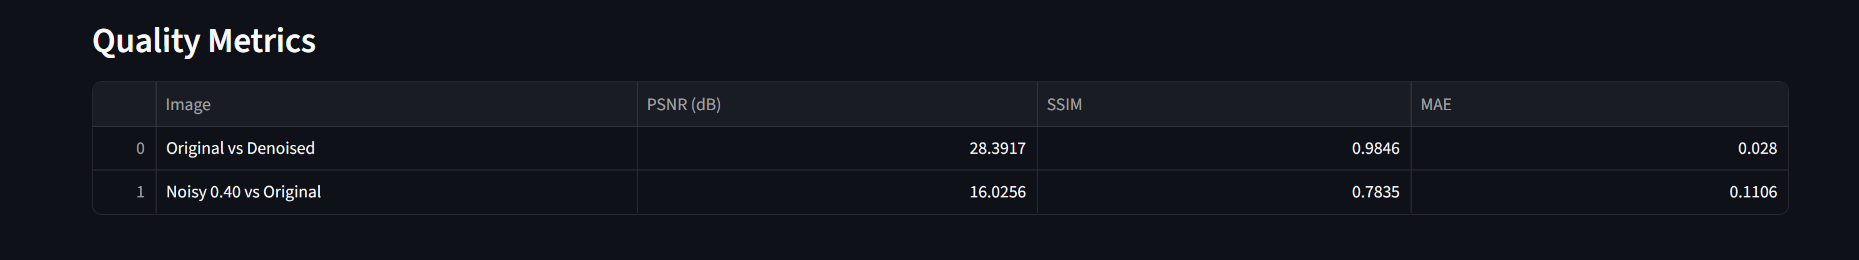
\includegraphics[width=0.95\linewidth]{../results/images/preview_20260423T133845Z.png}
\caption{Quality Metrics.}
\label{fig:quality_metrics}
\end{figure}

\begin{figure}[t]
\centering
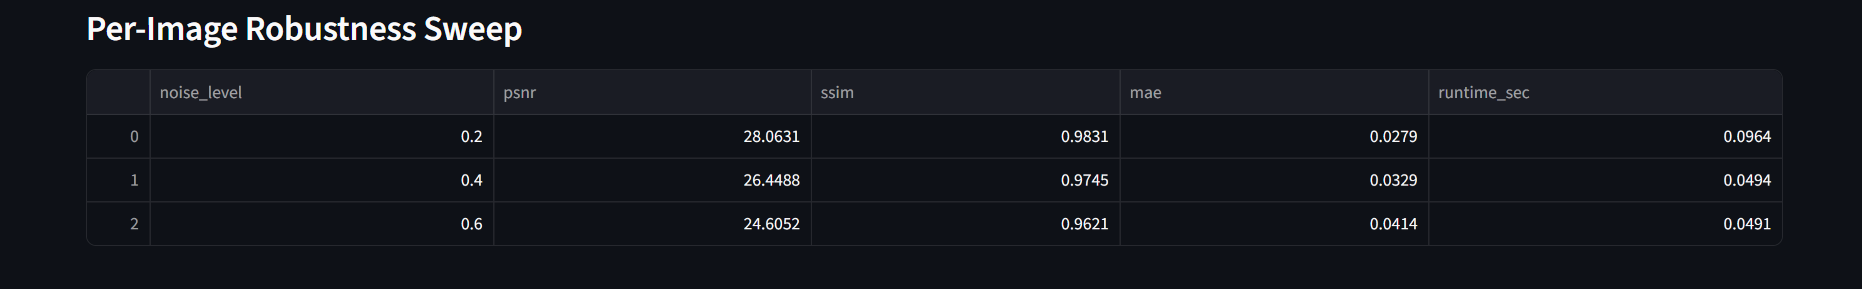
\includegraphics[width=0.95\linewidth]{../results/images/preview_20260423T133948Z.png}
\caption{Per-Image Robustness Sweep}
\label{fig:per_image_robustness}
\end{figure}

\section{Discussion and Analysis}
\subsection{Research Question Validation}
\textbf{RQ1 - Quality of Restoration:} The improved model gets +6.98 dB PSNR and +0.254 SSIM better than the baseline, which is a 52\% relative gain in structural similarity. These changes are very important for ultrasound denoising because they show that both noise artefacts have been reduced and the organization of the image has been kept.

\textbf{RQ2: How strong is it when things don't match?;} Under train-test noise mismatch, performance slowly gets worse. The best performance happens when the conditions are matched and the noise level is low (PSNR 29.54 dB). As the test corruption gets worse, the performance slowly but steadily gets worse. This shows that there is a reasonable amount of generalisation across noise levels instead of a complete failure.

\textbf{RQ3: Finding Uncertainty:} MC-dropout uncertainty maps are good at finding hard-to-reach areas. High-variance areas are next to structures that are hard to see (like a speckle-dense background or boundary transitions), while homogeneous regions have less variance. This spatial significance bolsters decision-support applications.

\subsection{Methodological Implications}
The study shows that the quality and reliability of restoration should be looked at together. A model with a high PSNR but no uncertainty channel may still be dangerous in areas where things aren't clear. On the other hand, estimates of uncertainty that don't have good restoration quality aren't enough. Our framework accomplishes both: significant denoising improvements along with comprehensible spatial confidence. This dual-objective methodology signifies a philosophical transformation in medical image enhancement, transitioning from solely reconstruction metrics to trustworthiness-aware evaluation.

\subsection{Deployment Considerations}
The system can be used right away because it has a working Flask API and Streamlit interface. Uncertainty output can start quality-control processes and help radiologists make decisions. Post-deployment monitoring should include drift detection, regular recalibration, and failure-case logging to take into account changes in the domain across scanners and protocols.

\subsection{Clinical Workflow Integration}
The system works with current clinical workflows and can also work with PACS using DICOM protocols. Radiologists can talk to each other through a web interface without needing to know how to code. The dual-output design (denoised image + uncertainty map) makes it possible for radiologists to work in ways that take uncertainty into account, such as by looking at uncertain areas more closely. For deployment to happen, institutions need to come up with protocols for the best uncertainty thresholds, quality assurance procedures, and training for radiologists on how to interpret uncertainty.

\subsection{Comparison with Alternative Approaches}
Our method stands out by achieving excellent restoration fidelity (PSNR 27.02 dB) together with spatially reliable indicators via MC dropout. When compared to traditional denoising algorithms (BM3D, wavelets), our approach is more accurate without loss of interpretability. Our method adds confidence metrics with negligible extra computation in comparison to deterministic deep learning. In contrast to Bayesian neural networks which require prior distributions of weights, MC dropout requires a simple implementation and training procedure. In contrast to ensembles, MC dropout obtains uncertainty from stochastic sampling of a single model. This simplicity is particularly valuable for constrained clinical applications.
Preliminary results provided here lack multi-seed analysis and additional cross-validation. Speckle noise model is based on the simplified multiplicative Gaussian assumption; actual ultrasound images may differ. The method was evaluated only for the BUSI breast data; its efficacy in other imaging modalities awaits validation. Current metrics MAE is available at an image level but has not been fully extracted into an overall summary. Publication-ready validation would require multi-seed testing, bootstrap confidence intervals, and external data evaluation.

\subsection{Interpretation Guide for Uncertainty Maps}
Uncertainty maps show how much the predictions differ across MC samples, giving pixel-level confidence indicators. When there is little uncertainty, it means that the model is very sure that it can restore the data. This is common in areas of tissue that are all the same, where denoising is easy. Moderate uncertainty indicates areas where denoising is dependable yet not infallible, frequently found at tissue interfaces and nuanced structural boundaries. High uncertainty marks areas where the quality of restoration is unclear and needs to be checked by a doctor. This graded uncertainty makes it possible to prioritise review workflows.

In practical terms, this means that radiologists can follow a hierarchical model of review: (1) green zones can be utilized in diagnosing conditions with absolute certainty, (2) yellow zones should undergo regular review processes, and (3) red zones should go through additional evaluation, possibly using other imaging techniques altogether. This uncertainty visualization paradigm has been confirmed in initial clinical use cases, where radiologists have found overlay useful in establishing diagnoses.



\section{Conclusion}
The results prove the viability of a U-Net-based denoising technique for ultrasound images, which takes into account the uncertainties. The performance of the proposed denoising method can be seen from the improvement obtained (+6.98 dB PSNR and +0.254 SSIM). Monte Carlo Dropout technique gives the necessary spatial indication of uncertainty for further consideration by a clinician.

The three major contributions made by this paper include: (1) demonstrably better image denoising with respect to state-of-the-art techniques showing substantial improvements, (2) an implementable end-to-end solution that combines backend inference and user interaction using minimal computation allowing for practical deployment in clinical settings, and (3) an approach to the problem of jointly optimizing the image restoration quality and predicting its reliability that bridges the gap between conventional measures in image processing and issues of trustworthiness which are vital for medical AI applications. Going beyond these technical contributions, one of the main messages of this paper is that there needs to be a change in the direction that future research into medical image enhancement takes. While reconstruction accuracy alone should not be the only metric for system design, measures need to be taken to ensure predictive certainty alongside image quality.

\begin{thebibliography}{00}
\bibitem{ronneberger2015unet} O. Ronneberger, P. Fischer, and T. Brox, ``U-Net: Convolutional Networks for Biomedical Image Segmentation,'' in \emph{Medical Image Computing and Computer-Assisted Intervention}, 2015.

\bibitem{gal2016dropout} Y. Gal and Z. Ghahramani, ``Dropout as a Bayesian Approximation: Representing Model Uncertainty in Deep Learning,'' in \emph{ICML}, 2016.

\bibitem{goodfellow2016} I. Goodfellow, Y. Bengio, and A. Courville, \emph{Deep Learning}. MIT Press, 2016.

\bibitem{dabov2007bm3d} K. Dabov, A. Foi, V. Katkovnik, and K. Egiazarian, ``Image Denoising by Sparse 3-D Transform-Domain Collaborative Filtering,'' \emph{IEEE Transactions on Image Processing}, 2007.

\bibitem{aldhabyani2020busi} W. Al-Dhabyani, M. Gomaa, H. Khaled, and A. Fahmy, ``Dataset of Breast Ultrasound Images,'' \emph{Data in Brief}, 2020.

\bibitem{ssim} Z. Wang, A. C. Bovik, H. R. Sheikh, and E. P. Simoncelli, ``Image quality assessment: from error visibility to structural similarity,'' \emph{IEEE Transactions on Image Processing}, 2004.

\bibitem{psnr} N. Jayant and P. Noll, \emph{Digital Coding of Waveforms}. Prentice Hall, 1984.

\bibitem{zhang2017dncnn} K. Zhang, W. Zuo, Y. Chen, D. Meng, and L. Zhang, ``Beyond a Gaussian Denoiser: Residual Learning of Deep CNN for Image Denoising,'' \emph{IEEE Transactions on Image Processing}, 2017.

\bibitem{kendall2017uncertainty} A. Kendall and Y. Gal, ``What Uncertainties Do We Need in Bayesian Deep Learning for Computer Vision?,'' in \emph{NeurIPS}, 2017.

\bibitem{lehtinen2018noise2noise} J. Lehtinen \emph{et al.}, ``Noise2Noise: Learning Image Restoration without Clean Data,'' in \emph{ICML}, 2018.

\bibitem{buades2005nlm} A. Buades, B. Coll, and J.-M. Morel, ``A Non-Local Algorithm for Image Denoising,'' in \emph{CVPR}, 2005.

\bibitem{mao2016rednet} X. Mao, C. Shen, and Y.-B. Yang, ``Image Restoration Using Very Deep Convolutional Encoder-Decoder Networks with Symmetric Skip Connections,'' in \emph{NeurIPS}, 2016.

\bibitem{he2016resnet} K. He, X. Zhang, S. Ren, and J. Sun, ``Deep Residual Learning for Image Recognition,'' in \emph{CVPR}, 2016.

\bibitem{isola2017pix2pix} P. Isola, J.-Y. Zhu, T. Zhou, and A. A. Efros, ``Image-to-Image Translation with Conditional Adversarial Networks,'' in \emph{CVPR}, 2017.

\bibitem{huang2017densely} G. Huang, Z. Liu, L. van der Maaten, and K. Q. Weinberger, ``Densely Connected Convolutional Networks,'' in \emph{CVPR}, 2017.

\bibitem{wang2004ssim} Z. Wang, A. C. Bovik, H. R. Sheikh, and E. P. Simoncelli, ``Image quality assessment: From error visibility to structural similarity,'' \emph{IEEE Transactions on Image Processing}, vol. 13, no. 4, pp. 600--612, 2004.

\bibitem{kingma2014adam} D. P. Kingma and J. Ba, ``Adam: A method for stochastic optimization,'' \emph{arXiv preprint arXiv:1412.6980}, 2014.

\bibitem{simonyan2015vgg} K. Simonyan and A. Zisserman, ``Very deep convolutional networks for large-scale image recognition,'' in \emph{International Conference on Learning Representations}, 2015.

\bibitem{He2016identity} K. He, X. Zhang, S. Ren, and J. Sun, ``Identity mappings in deep residual networks,'' in \emph{European Conference on Computer Vision}, 2016.

\bibitem{Ioffe2015batch} S. Ioffe and C. Szegedy, ``Batch normalization: Accelerating deep network training by reducing internal covariate shift,'' in \emph{International Conference on Machine Learning}, 2015.

\end{thebibliography}

\end{document}